\documentclass{ltjsbook}
\usepackage{docmute} 
\usepackage{../../myStyle} 

\begin{document}
\chapter{多次元尺度構成法}
\label{x15_MDS}
今回は\keyterm{多次元尺度構成法}{たじげんしゃくどこうせいほう}{Multi-Dimensional Sacling; MDS}について解説します。
ここまで分散共分散行列を分解するところから，クロス表のような\keyterm{名義尺度水準}{めいぎしゃくどすいじゅん}のデータを分解するところまでやってきました。

多次元尺度構成法は，分散共分散行列を扱う線形モデルよりはやや仮定が緩く，また数量化のように解析者が数字を与えることを目的にするというよりは，その名の通り尺度を作ろうとしているという意味で心理学的・心理測定的なモデルだといえるでしょう。

私たちが単位もない不確かなものを対象にしながらもそれを測定するモノサシをつくることができるのは，2つの対象にたいしてその比較をして一方が他方よりも大である，ということが言えるからでしょう。
記号を使って言えば，$x$と$y$を比べて$x \succeq y$である，ということから，尺度上の値$p \ge q$を対応させるということが，尺度を作るということです\footnote{経済学では学問の最初の段階で，財を源とした集合に対する二項関係$x \circ y$を定義し，それを効用関数$u$で実数領域に写像して$u(x) \ge u(y)$を考える，といった基本的な原理を抑えます。心理学ではなぜか，「集合」「元」「二項関係」という基本的な比較の要素について考えることなく，その分析ツールだけがどんどんと発展してきています。}。
このとき比較する2つが重さや広さのような物理的なものであればわかりやすいですし，「痛み」や「喜び」といった心理的な要素であっても構いません。あるいは「より賛成」といった態度表明のようなものでも良いかもしれません。
この比較から出てくる関係は，分散共分散や相関係数のように強い線形の過程を置かなくても，より緩やかに\keyterm{距離}{きょり}{distance}という考え方で表現されます\footnote{後述しますが，相関係数も距離の一種と考えられます。}。

MDSは距離行列を固有値分解するモデルです。それではこの方法について内容を見ていきましょう。

\section{多次元尺度構成法}
Rにはサンプルデータとして\texttt{eurodist}というヨーロッパ各地の都市間距離のデータが用意されています。表\ref{tbl::15_01}にその一部を示します。

\begin{table}[ht]
	\centering
	\caption{ヨーロッパ都市間距離データの一部}
	\begin{tabular}{l|rrrrrr}
		          & Athens & Barcelona & Brussels & Calais & Cherbourg & Cologne \\
		\hline
		Athens    & 0      &           &          &        &           &         \\
		Barcelona & 3313   & 0         &          &        &           &         \\
		Brussels  & 2963   & 1318      & 0        &        &           &         \\
		Calais    & 3175   & 1326      & 204      & 0      &           &         \\
		Cherbourg & 3339   & 1294      & 583      & 460    & 0         &         \\
		Cologne   & 2762   & 1498      & 206      & 409    & 785       & 0       \\
		\hline
	\end{tabular}
	\label{tbl::15_01}
\end{table}

元のデータは$21 \times 21$のサイズです。表から，たとえばアテネ(Athens)とバルセロナ(Barcelona)の距離が3313km，と言うことが読み取れます。表の右上が空白になっていますが，これは\keytermL{距離行列}{きょりぎょうれつ}が\keytermL{対称行列}{たいしょうぎょうれつ}なので，ムダな情報を表示しないようにしているからです。アテネとバルセロナの距離は，バルセロナとアテネの距離に等しいですからね。

さて距離行列はこのように，\keytermL{正方行列}{せいほうぎょうれつ}ですから，\keytermL{固有値分解}{こゆうちぶんかい}をすることで\keytermL{基底}{きてい}を求めることができます。基底は座標を形成する基本単位ですから，それを使って各変数の位置にあたる座標を計算できます\footnote{厳密には距離行列$\bm{D}$そのものではなく，それを二重中心化した行列の固有値分解になりますが，本質的には変わりません。詳しくは\textcite{Okada19940115}などを参照のこと。}。このように距離行列から座標を求めて，変数をプロットすることで変数間関係を可視化する手法のことを\keyterm{多次元尺度構成法}{たじげんしゃくどこうせいほう}{Multi-Dimensional Scaling: MDS}と言います。

試しに\texttt{eurodist}データをMDSで2次元プロットしてみましょう。
これを実行するコードは簡単で，\texttt{eurodist}データのようにデフォルトで組み込まれている\texttt{cmdscale}関数を使います。

\begin{lstlisting}[language=C++,label={code:x15_01},caption={計量MDSの実践と描画}]
library(ggrepel)
# MDSを実行
result.MDS1 <- cmdscale(eurodist,k=3)
# y軸反転させつつ描画
g <- result.MDS1 %>%
  as.data.frame() %>%
  dplyr::mutate(label = rownames(.)) %>%
  ggplot(aes(x = V1, y = V2, label = label)) +
  geom_point() +
  geom_text_repel() +
  xlim(-2500, 2500) +
  ylim(2500, -2500) +
  xlab("dim 1") +
  ylab("dim2")
\end{lstlisting}

\paragraph{コード解説}
\begin{description}
	\item[1行目] \verb|ggplot2|でラベルをプロットするときに，綺麗な配置にしてくれる\verb|ggrepel|パッケージを使います。このコードを実行するときに持っていない人は，インストールしておいてください。
	\item[3行目] \verb|cmdscale|関数に\verb|eurodist|データを与えています。\verb|k=3|は3次元解を出すように指定しています。地球は球体ですから，地球上の地理は3次元で表現できますよね。
	\item[5-14行目] \verb|ggplot2|による描画です。結果オブジェクトである\verb|result.MDS|をデータフレームにし，行の名前になっていた都市名を変数として格納したのち，散布図のようにプロットしています。
\end{description}

\begin{figure}[ht]
	\begin{center}
		\includegraphics[width=0.8\linewidth,keepaspectratio]{../images/15_MDS/Rplot15_01.png}
		\caption{MDSのプロット}
		\label{fig:15_01}
	\end{center}
\end{figure}

図\ref{fig:15_01}をみると，上の方にストックホルム(Stockholm)があって，右下にアテネが，中央にパリ(Paris)が・・・といった配置になっています。地球上の位置と完全に一致しているとは言えませんが，それでも概ねうまくプロットできていますね\footnote{完全に一致しない理由は，地球が球面であるのに対し平面にプロットしたから，と言うのもあります。}。このように，距離関係だけから地図を作ることができるというのが，MDSという手法なのです。

\section{距離と心理学のデータ}
\label{distance}
MDSは距離関係だけから地図を作る方法でした。因子分析は相関関係から次元を作る方法でした。この2つの手法はとても似ています。というのも，相関関係と言うのが変数と変数の近さ・遠さ，つまり距離を表しているとも言えるからです。
あらためて\keyterm{距離}{きょり}{distance}とは何かを考えてみましょう。2点$x,y$の距離を$d(x,y)$とすると，距離とよばれる数字の条件は次のようになります。
\begin{description}
	\item[非負性] $d(x,y)\ge 0$
	\item[非退化性] $d(x,y)=0 \Leftrightarrow x=y$
	\item[対称性] $d(x,y)=d(y,x)$
	\item[三角不等式] $d(x,z) + d(z,y) \ge d(x,y)$
\end{description}
もっとも一般的に使われるのはユークリッド距離で，2次元座標$(x_1,y_1),(x_2,y_2)$があった時のユークリッド距離は次のように計算します。
\[ \sqrt{(x_1-x_2)^2+(y_1-y_2)^2} \]
3次元座標$(x_1,y_1,z_1),(x_2,y_2,z_2)$の場合は項を増やすだけです。
\[ \sqrt{(x_1-x_2)^2+(y_1-y_2)^2+(z_1-z_2)^2} \]
このようにして計算される距離ですが，上の条件を考えると何も二乗してルートを取らなくても絶対値を足し合わせるような方法でも構いません。たとえば2次元座標の場合は，次のような計算でもいいのです。
\[ |x_1-x_2|+|y_1-y_2| \]
現にこのような距離のことを\keyterm{マンハッタン距離}{まんはったんきょり}{Manhattan distance}といいます。二乗ではなくn乗してn乗根をとる，という形で一般化することもできます。
\[ d(x,y) = \left( \sum_{i=1}^n |x_i - x_j|^p\right)^{\frac{1}{p}} \]
これは\keyterm{ミンコフスキー距離}{みんこふすきーきょり}{Minkowski distance}という名前がついています。他にもマキシマム距離，バイナリ距離，チェビシェフの距離，キャンベラ距離などがあり，いずれもRの\texttt{dist}関数のオプションで選ぶことができますので，ヘルプなどを参照してみてください。

また，相関係数$r_{ij}$は$-1 \le r_{ij} \le +1$の範囲にありますが，この絶対値から$1-|r_{ij}|$とするとこれも距離の条件に当てはまります。どの程度類似しているかというのも，距離と考えることができるのです。

ここまでは数学的な距離のバリエーションでしたが，次に心理学的な意味に目を向けてみましょう。
距離とは類似度でもありますから，何を距離と見なすかによって，さまざまな心理学的刺激がデータを形作ることになります。

たとえば評定尺度で，n個の項目で何らかの評価をしてもらったとします。$x_{ij}$を$i$番目の項目における対象$j$の評定値だとすると，
$d(j,k) = \sqrt{\sum_{i=1}^N (x_{ij}-x_{ik})^2 }$とすれば対象の類似度が計算できます。
ほかにも何らかの刺激A,Bについて，AかBかの判断をさせた時に混同してしまった混同率や，単語と単語の連想価，刺激の汎化勾配，反応潜時，ソシオメトリックなデータなど，いろいろなものが「類似しているかどうか」の指標として使えます\footnote{これらデータの例に関しては\textcite{Takane198002}のPp.14--27を参照してください。}。尺度評定よりも，具体的な2つの刺激が似ているかどうかの反応の方がやりやすい，というのは誰しも実感としてわかることではないかと思います。

類似度のデータが得られれば，それを距離と見做してMDSにかければ，変数間の関係を地図に描くことができるわけです。このように応用可能な領域が非常に広いことも，MDSの利点であると言えるでしょう。

\section{非計量多次元尺度法}

さて心理学的なさまざまな刺激が，MDSによって可視化できるということがわかってきました。距離行列が構成できれば，後の分析は何とでもできるわけです。
ただし，この場合の距離行列とは，間隔尺度水準以上であることが必要です。
しかし心理学的な刺激に対する反応をデータ化する時は，同時に被験者はそこまで鋭敏に反応しているのか，いいかえれば本当に間隔尺度水準以上の精度で判断できているのかな，という人間側の問題が気になりますね。そこまで人間は鋭敏無反応をしていないかもしれません。

でも大丈夫。MDSは仮定を緩めたモデルがあります。\keyterm{非計量的多次元尺度構成法}{ひけいりょうてきたじげんしゃくどこうせいほう}{Non-Metric Multi-Dimensional Scaling}と呼ばれる手法がそれです。非計量MDSでは，対象$j$と$k$の類似度を$\delta_{jk}$とし，分析によって埋め込む多次元空間での距離を$d_{jk}$とすると，

$$ \delta_{jk} > \delta_{lm} \mbox{ならば}d_{jk}\le d_{lm} $$

のように，イコールではなく順序関係だけ保持して座標を求めます。この手法では，元データが順序尺度水準程度の情報しか持っていなくても地図を描くことができるのです。人間の判断はせいぜいが順序尺度ぐらいですから，「より類似している($\delta_{jk} > \delta_{lm}$)」のであれば「より近くにある($d_{jk}\le d_{lm} $)」というぐらいの配置の方が良いかもしれません。


表\ref{tbl::15_01}に示したような物理的距離であれば，間隔尺度水準の情報であることは間違いありません。その場合には，最初に示した固有値分解による手法を使います。これは非計量MDSに対して，\keyterm{計量的多次元尺度構成法}{けいりょうてきたじげんしゃくどこうせいほう}{Metric Multi-Dimensional Scaling}と呼ばれています。

\subsection{非計量多次元尺度法の例}

心理学ではデータの性質上，非計量MDSのほうが便利なことが多いでしょう。計量MDSでも非計量MDSでも，Rでは簡単な関数で実行できます。ここでは\verb|MASS|パッケージに含まれる\verb|isoMDS|関数を使って実践してみます。

使うデータは\verb|M1score2021.csv|とします\footnote{ファイルはシラバスのサイトからダウンロードできます。}。ファイル名からお察しいただけるように，M-1グランプリの評定をデータ化したものです\footnote{念のために解説しておきますが，M-1グランプリとは2001年から始まった漫才の賞レースの1つで，年末に年間チャンピオンが決定します。開催年ごとにルールが少し変わることもありますが，基本的には予選を勝ち抜いた10組の漫才師が4分間のネタを披露し，6-7名の審査員が100点満点で採点します。点数の上位3組が決勝戦を行い2本目のネタを披露，投票によりチャンピオンが選出されるという流れです。2021年はオール巨人，富澤たけし，塙宣之，立川志らく，中川礼二，松本人志，上沼恵美子が審査員で，最終的には錦鯉がチャンピオンになりました。このデータセットは1本目のネタについての採点を2001年から集めたものになります。}。2021年度のスコアは表\ref{tbl:x15_m1}でした。

\begin{table}[ht]
	\centering
	\caption{M-1グランプリ2021の採点結果}
	\begin{tabular}{l|cccccccc}
		\hline
		演者        & 巨人 & 富澤 & 塙  & 志らく & 礼二 & 松本 & 上沼 \\
		\hline
		モグライダー    & 91 & 93 & 92 & 89  & 90 & 89 & 93 \\
		ランジャタイ    & 87 & 91 & 90 & 96  & 89 & 87 & 88 \\
		ゆにばーす     & 89 & 92 & 91 & 91  & 93 & 88 & 94 \\
		ハライチ      & 88 & 90 & 89 & 90  & 89 & 92 & 98 \\
		真空ジェシカ    & 90 & 89 & 92 & 94  & 94 & 90 & 89 \\
		オズワルド     & 94 & 95 & 95 & 96  & 96 & 96 & 93 \\
		ロングコートダディ & 89 & 90 & 93 & 95  & 95 & 91 & 96 \\
		錦鯉        & 92 & 94 & 94 & 90  & 96 & 94 & 95 \\
		インディアンス   & 92 & 91 & 93 & 94  & 94 & 93 & 98 \\
		もも        & 91 & 90 & 91 & 96  & 95 & 92 & 90 \\
		\hline
	\end{tabular}
	\label{tbl:x15_m1}
\end{table}


M-1の採点は審査員各自の主観に基づいて行われ，得点の絶対値はそれほど重要ではないかもしれません。すなわち，松本人志の80点が上沼恵美子の80点と同じぐらいの面白さを評価しているか，ということについては真偽判断ができないでしょう。それでも各審査員の中での相対的評価には，一貫性がありそうです。すなわちある審査員が漫才師Aに80点，漫才師Bに85点をつけたのならBの方が面白かったということでしょうし，漫才師Cが83点なら$A<C<B$という順序はあると思われます。つまり\keytermL{順序尺度水準}{じゅんじょしゃくどすいじゅん}程度の質はあると仮定することに無理はなさそうです。

そこでこのデータをもとに，10組の漫才師の類似度を計算します。類似度はユークリッド距離を用いることにします。ユークリッド距離は既に述べたように差分の二乗を総和して平方根を取ったものですが，具体的な数字で見た方がわかりやすいかもしれませんので，表\ref{tbl:x15_distance}を用意しました。
\begin{table}[ht]
	\centering
	\caption{距離の計算}
	\begin{tabular}{l|rrrrrrrr}
		\hline
		       & 巨人 & 富澤 & 塙  & 志らく & 礼二 & 松本 & 上沼 & 総和  \\
		\hline
		モグライダー & 91 & 93 & 92 & 89  & 90 & 89 & 93 & 637 \\
		ランジャタイ & 87 & 91 & 90 & 96  & 89 & 87 & 88 & 628 \\
		\hline
		差分     & 4  & 2  & 2  & -7  & 1  & 2  & 5  & 9   \\
		差分の二乗  & 16 & 4  & 4  & 49  & 1  & 4  & 25 & 103 \\
		\hline
	\end{tabular}
	\label{tbl:x15_distance}
\end{table}
表\ref{tbl:x15_distance}にモグライダーとランジャタイの二組だけ取り出し，これで計算例を見てみます。それぞれの得点の差分，その二乗を計算し，それを総和したところ$103$という値になっています。これの平方根を取ったもの，すなわち$\sqrt{103}=10.14889$がこの二組の距離，すなわち非類似度ということになります。この計算を全ての組み合わせについて計算してくれるのが，\verb|dist|関数なのです。

\begin{lstlisting}[language=C++,label={code:x15_02},caption={距離行列の計算}]
dat <- read_csv("M1score2021.csv")
dat.mat <- dat %>%
  dplyr::filter(年代 == 21) %>%
  arrange(ネタ順) %>% 
  dplyr::select(-年代, -ネタ順) %>%
  pivot_longer(-演者) %>%
  na.omit() %>%
  pivot_wider(id_cols = 演者, 
  			  names_from = name,
			  values_from = value) %>%
  as.matrix()
rownames(dat.mat) <- dat.mat[, 1]
dat.mat <- dat.mat[, -1] %>%
  dist()
\end{lstlisting}

\paragraph{コード解説}
\begin{description}
	\item[1行目] データファイルを読み込み，\verb|dat|オブジェクトに格納します。
	\item[2-9行目] 必要なデータだけに絞り込む操作です。流れを解説しますが，他のやり方でもいいですしできあがったものが何かだけわかれば結構です。
	      \begin{description}
		      \item[3行目] 2021年のデータだけに絞り込みます。
		      \item[4行目] ネタ順に並び替えています。
		      \item[5行目] 年代変数とネタ順変数はもういらないので削除してしまっています。
		      \item[6行目] ロング型に変換しています。これで演者-審査員-採点のデータセットができます。
		      \item[7行目] 欠測値を除外しています。実はこれがこの操作の目的で，というのも過去の審査データも入っているものですから，過去の審査員も大量に変数として含まれていて，それらが欠測値になってしまっていたのです。
		      \item[8-10行目] 元のワイド型に戻しています。
		      \item[11行目] 以下の行列処理のため，\verb|data.frame|型から\verb|matrix|型に変換しています。
	      \end{description}
	\item[12行目] 変数として一列目に演者名が入っていますが，これを行列の行名に入れています。\verb|matrix|型は行名・列名をデータの外に持つのです。
	\item[13-14行目] 変数としての演者名を除いて，パイプで\verb|dist|関数に入れ，距離行列を作っています。
\end{description}
できた距離行列は，表\ref{tbl:x15_distMat}のようになっています。モグライダーとランジャタイの距離が，先ほどの例で計算した値と一致していることを確認してください。またこれは\keytermL{正方対称行列}{せいほうたいしょうぎょうれつ}ですから下三角だけ表示しておいます。また，対角が$0$になっています。自分自身との距離はゼロだからです。

\begin{table}[ht]
	\centering
	\caption{演者の非類似度行列(演者名は略記)}
	\begin{tabular}{l|ccccccccccc}
		\hline
		    & モグ     & ラン     & ゆに     & ハラ     & 真空     & オズ    & ロン    & 錦鯉    & インデ   & もも    \\
		\hline
		モグ  & 0.000  &        &        &        &        &       &       &       &       &       \\
		ラン  & 10.149 & 0.000  &        &        &        &       &       &       &       &       \\
		ゆに  & 4.583  & 9.165  & 0.000  &        &        &       &       &       &       &       \\
		ハラ  & 7.937  & 12.806 & 7.616  & 0.000  &        &       &       &       &       &       \\
		真空  & 8.660  & 7.483  & 7.071  & 11.832 & 0.000  &       &       &       &       &       \\
		オズ  & 12.490 & 15.652 & 12.207 & 14.933 & 11.000 & 0.000 &       &       &       &       \\
		ロン  & 9.381  & 11.446 & 6.403  & 9.110  & 7.416  & 9.487 & 0.000 &       &       &       \\
		錦鯉  & 8.485  & 15.264 & 8.307  & 10.909 & 10.247 & 7.071 & 7.874 & 0.000 &       &       \\
		インデ & 9.381  & 14.107 & 8.062  & 8.660  & 9.950  & 8.124 & 4.472 & 6.325 & 0.000 &       \\
		もも  & 10.100 & 9.110  & 8.307  & 12.207 & 3.606  & 8.718 & 6.782 & 9.592 & 8.718 & 0.000 \\
		\hline
	\end{tabular}
	\label{tbl:x15_distMat}
\end{table}
あとはこの距離行列を\verb|isoMDS|関数に渡すだけです。\verb|isoMDS|関数は引数として，何次元の解を求めるかを設定できます。地理データであれば2,3次元から作られていることは明らかですが，この評価が何次元かは事前にわかりません。何次元にするかの指標として，\textcite{kruskal1964}は\verb|Stress|と呼ばれる値を次のように定義しました。

\[ Stress = \sqrt{\frac{\sum(d_{ij} - \delta_{ij}^2)}{\sum d_{ij}^2}} \]

つまり実際のデータの距離$d_{ij}$と，MDSで作られる空間上の座標から計算される距離$\delta_{ij}$の全体的な距離を当て嵌まりの指標と考えていることになります。
これを目安に，次元数を1から7まで変化させながら，Stress値がどうなるかを表したのが図\ref{fig:15_02}になります\footnote{どうして7までか，というと評定者が7名だからです。7名それぞれの評価次元があると考えると，この距離空間の中には最大7次元あるはずですから。あるいは10組の演者がいますから，組み合わせの自由度から考えて9次元まで試してもいいと思います。}。

\begin{figure}[ht]
	\begin{center}
		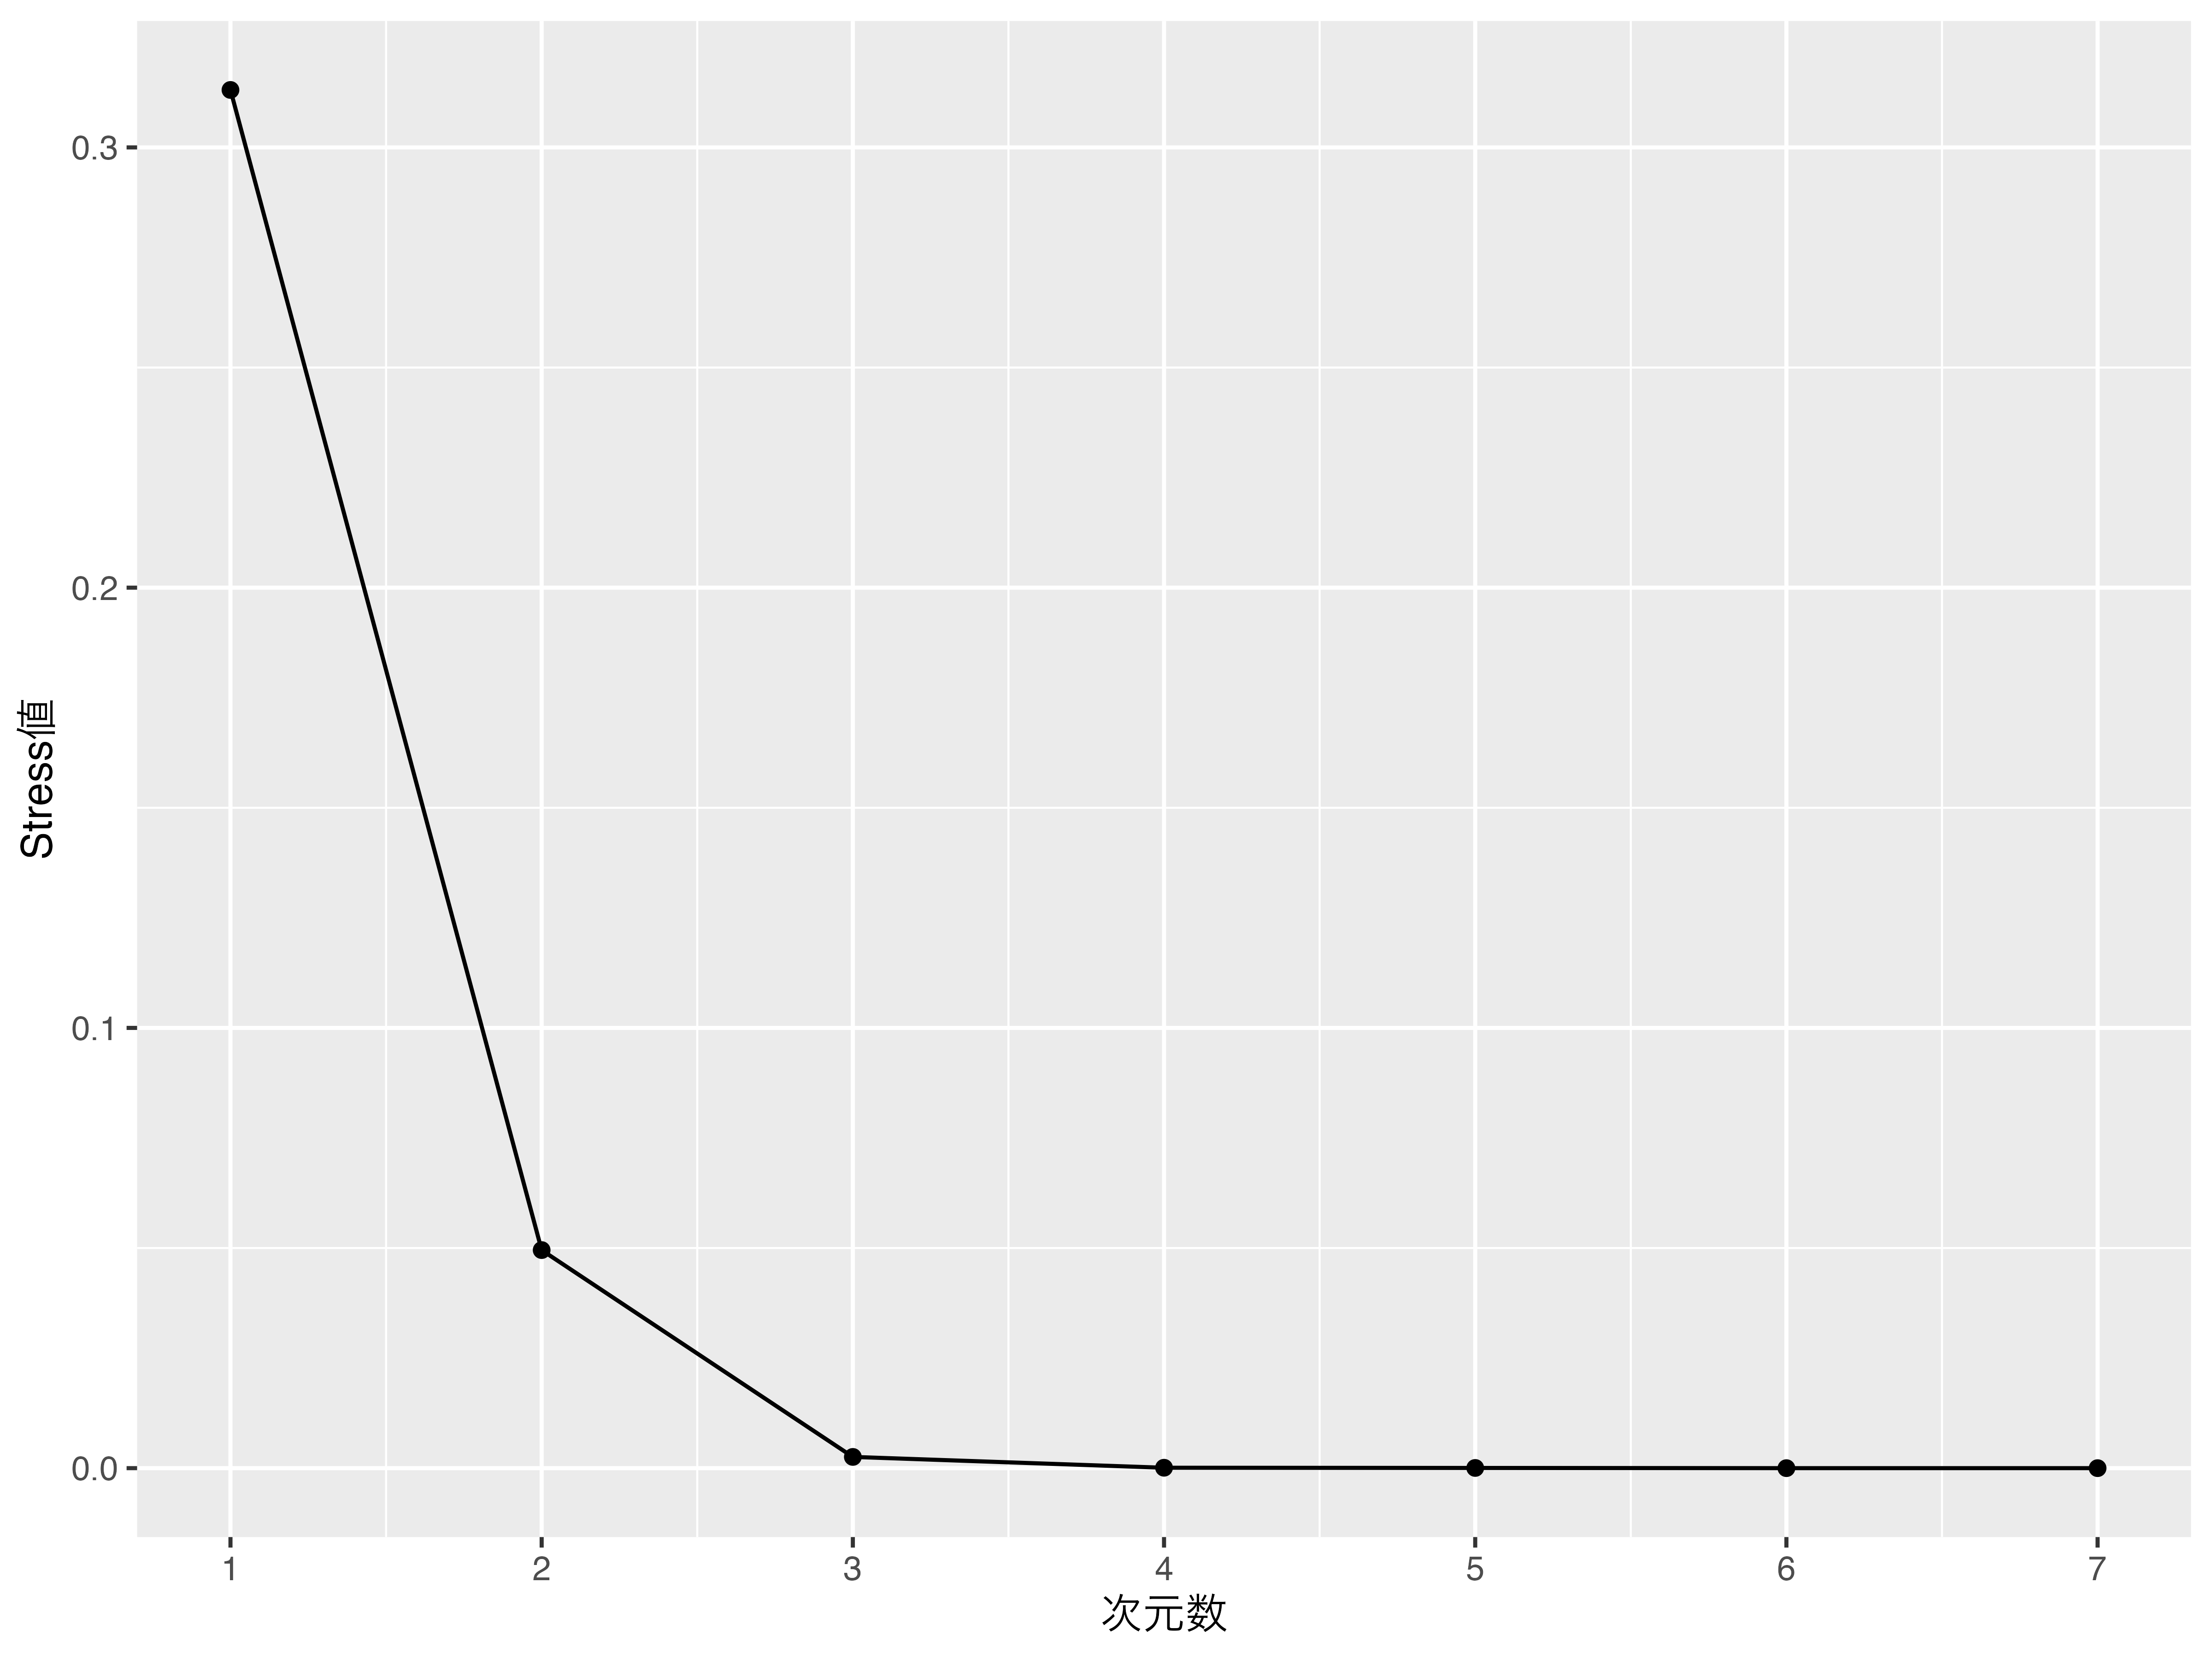
\includegraphics[width=0.8\linewidth,keepaspectratio]{../images/15_MDS/Rplot15_02.png}
		\caption{Stress値の減衰}
		\label{fig:15_02}
	\end{center}
\end{figure}

まるで因子分析の\keytermL{スクリープロット}{すくりーぷろっと}のようですね。横軸に次元数，縦軸にStress値を置いた折れ線グラフですが，当然のことながら反映させるMDS空間の次元数が増えるとデータとの距離が縮んでいきます。
\textcite{kruskal1964multidimensional}の基準によれば，Stress値は表\ref{tbl:x15_stress}のように評価できます。この基準でいくと，今回は2次元で4.9\%(0.0049534)ですから，2次元解でOKとしましょう。

\begin{table}[ht]
	\centering
	\caption{Stress値の評価}
	\begin{tabular}{cc}
		Stress           & Goodness of Fit \\\hline
		20\%             & poor            \\
		10\%             & fair            \\
		5\%              & good            \\
		$2\frac{1}{2}$\% & excellent       \\
		0\%              & ``perfect''     \\\hline
	\end{tabular}
	\label{tbl:x15_stress}
\end{table}

演者をプロットしたのが図\ref{fig:15_03}です。東西南北というか，上下左右の軸に特に意味はありませんから，因子分析のように因子軸の解釈や命名をすることはありません。近くにプロットされた対象は評価が似ていたんだな，ということがわかりますし，相対的な位置関係から，「ハライチとももは芸風が真逆だな」とか「ロングコートダディは中心に近いから中庸的な笑い，悪く言えばキャラが立ってないんだな」といったことが読み取れます。
\begin{figure}[ht]
	\begin{center}
		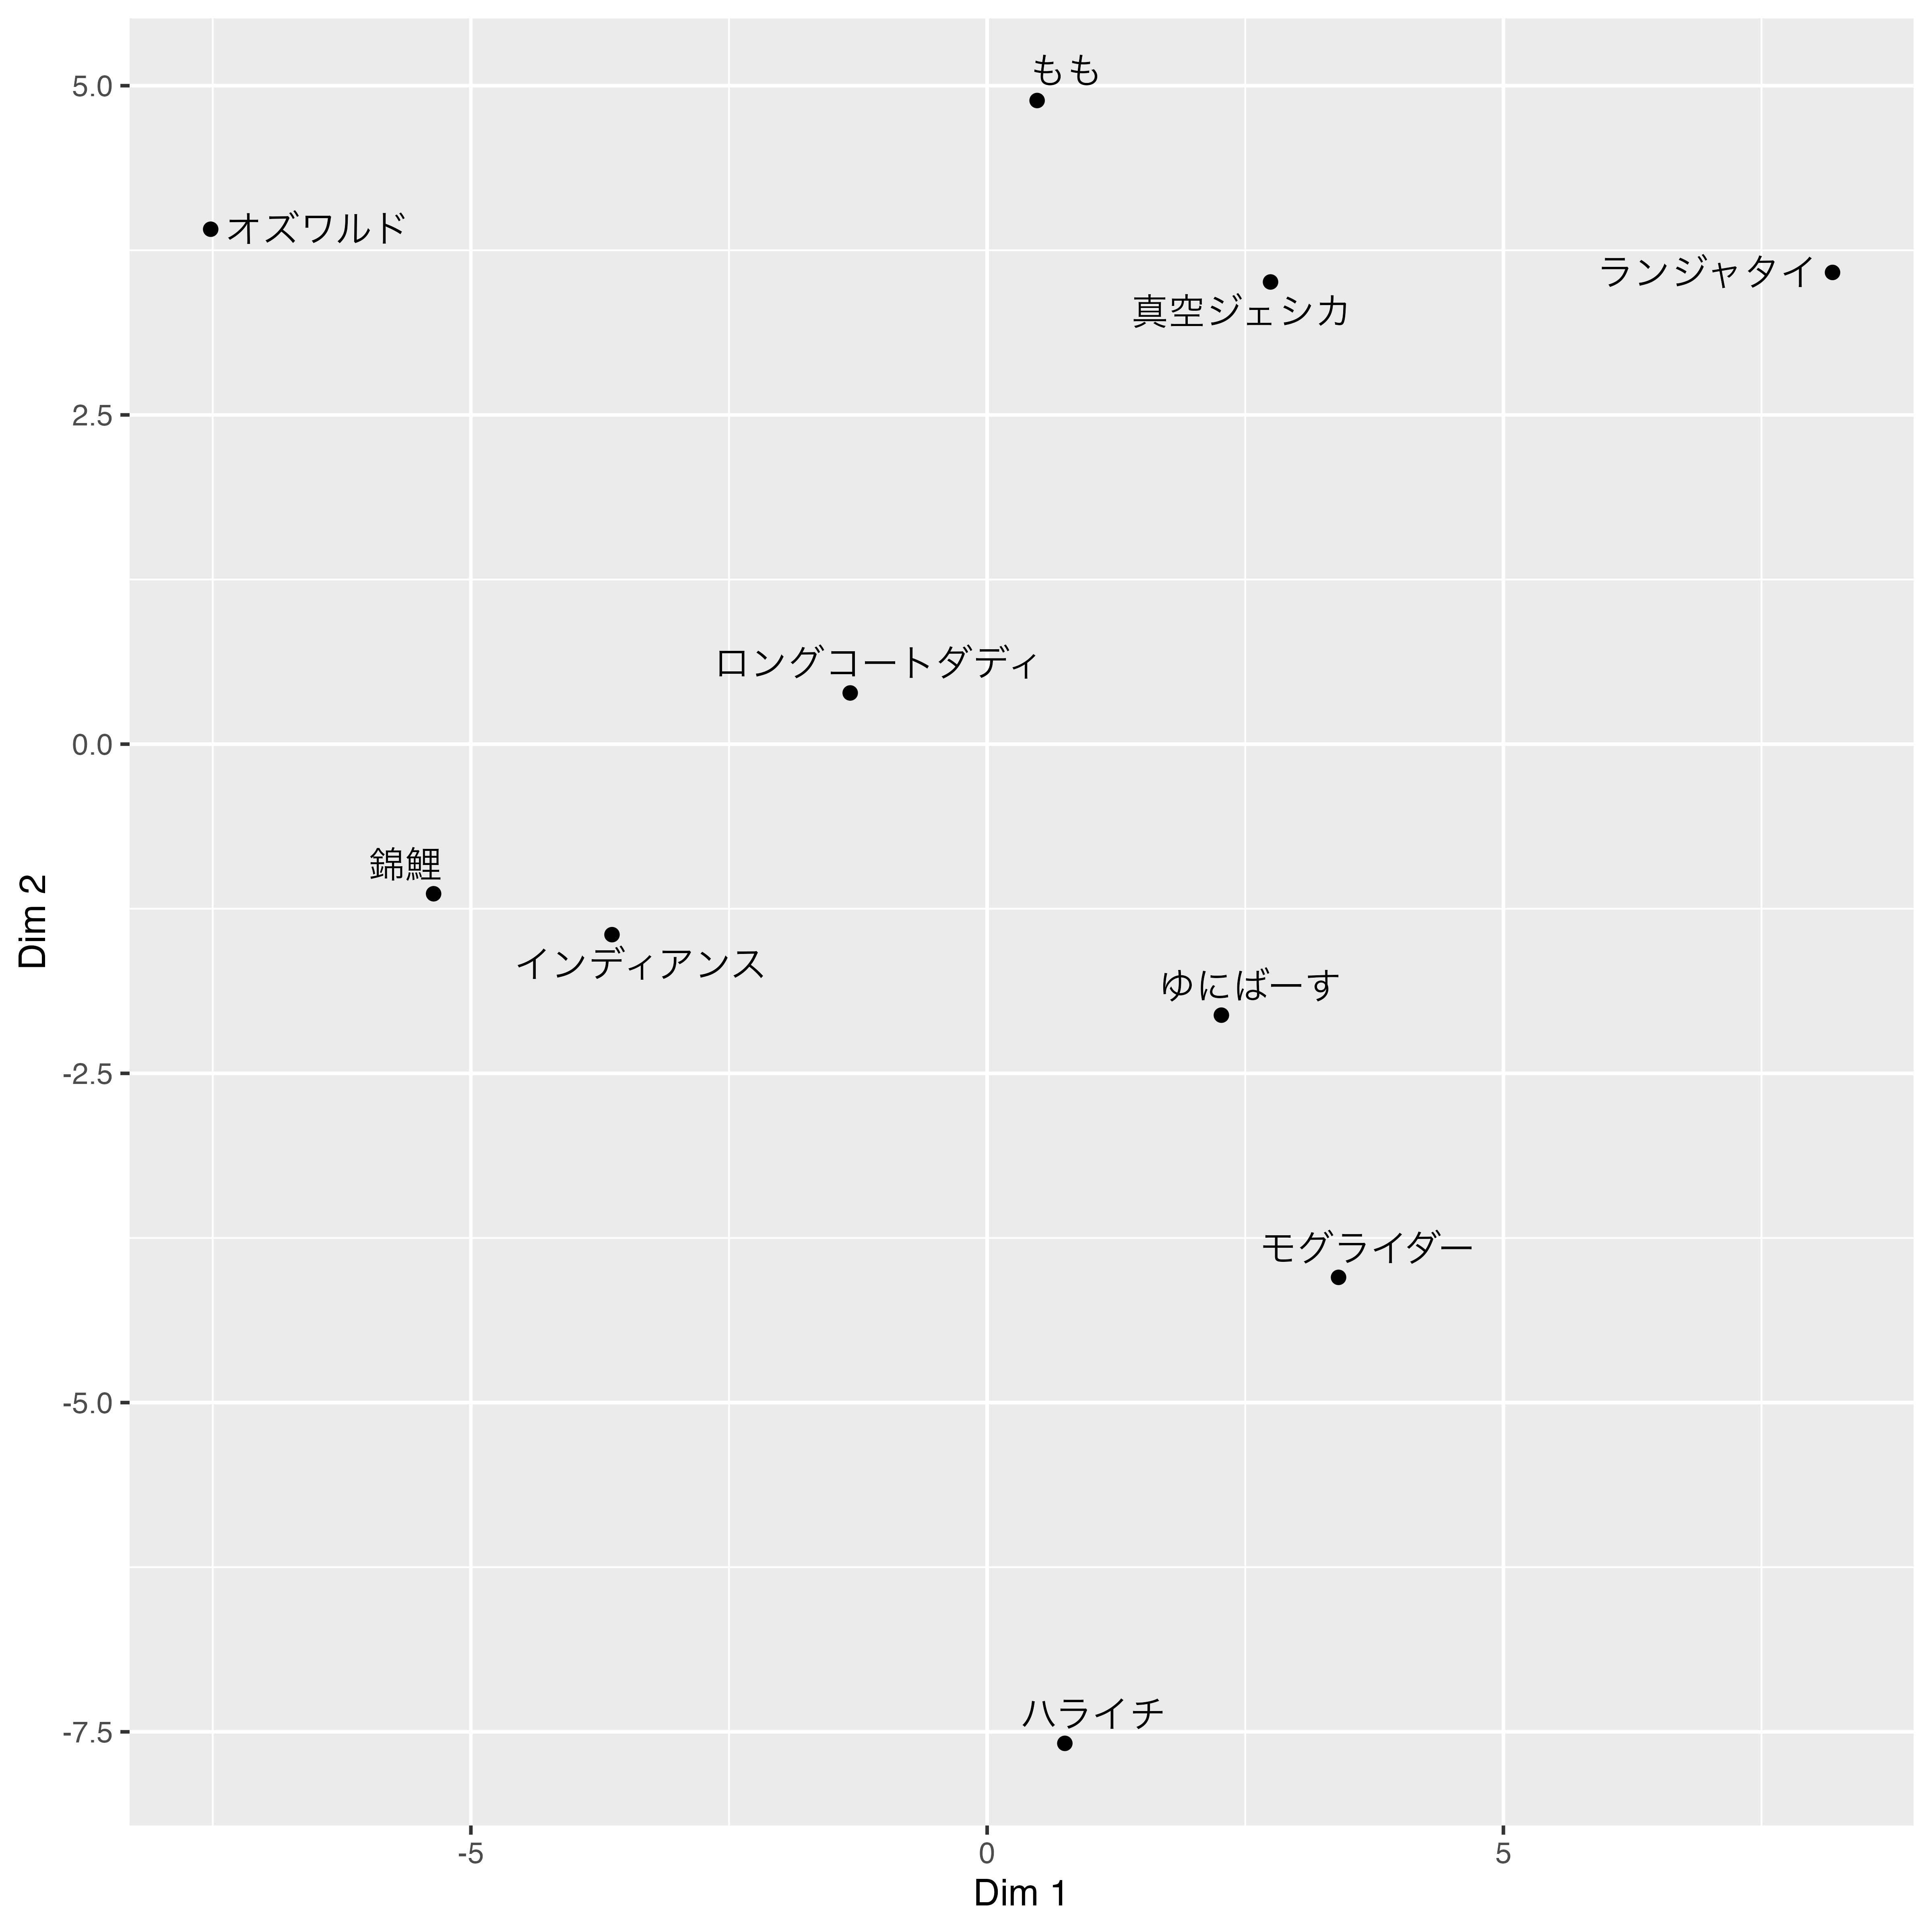
\includegraphics[width=0.8\linewidth,keepaspectratio]{../images/15_MDS/Rplot15_03.png}
		\caption{非計量MDSのプロット}
		\label{fig:15_03}
	\end{center}
\end{figure}
この図\ref{fig:15_01}や図\ref{fig:15_03}のようにMDSで作られた座標のことを特に\keyterm{布置}{ふち}{configure}といいます。特に非計量MDSは優劣・大小関係という順序尺度水準の評定だけからでも，その空間的な特徴を描くことができますから，心理尺度のもつ仮定や測定モデルを考える必要がないため，今後その重要性が再発見されていくのではないかと思います。

\section{多次元尺度法の展開}
多次元尺度構成法で作られた地図は，対象をプロットした地図です。
地図には，その上に何か書き込んだり，地形の図に天気図を重ねるように複数の地図を重ねて表現したりできます。
多次元尺度構成法にも，このような応用モデルがいろいろ考えられています。ここでいくつかの発展的なMDSモデルを見てみましょう。

\paragraph{prefmap}類似度空間の上に，個々人の理想点を追加する方法です。個人の好みpreferenceをマッピングする方法なので，\keyterm{Preference Mapping}{Preference Mapping}{}と呼ばれています。個人$i$が対象$j$について，好みの程度を$s_{ij}$と評価したとします。対象$1,2,...j...,M$は別途類似度評定によって，MDSのつくった地図上にプロットされているとします。ここで個人$i$と対象$j$との地図上の距離$d_{ij}^2$に対して，次の回帰式を考えます。
\[ s_{ij} = a_i d_{ij}^2 + b_i + e_{ij} \]
つまり，個人$i$と対象$j$の距離を使って，好みの程度$s_{ij}$を予測するモデルを作り，誤差がもっとも小さくなる点に個人$i$をプロットするのです。こうすることで，対象とそれを評価する人を一枚の地図に表現すると言うことができます。

例えば先ほどのM-1の例ですが，私の採点では表\ref{tbl:x15_kosugiRatio}のようになりました\footnote{ランジャタイは何が面白いのかわからなかった。モグライダーはもっと評価されるべき。ハライチも良かったですね，ちょっと時間オーバーしたっぽいけど。}。
\begin{table}[ht]
	\centering
	\caption{著者の評定}
	\begin{tabular}{cc}
		演者        & 採点 \\\hline
		モグライダー    & 90 \\
		ランジャタイ    & 60 \\
		ゆにばーす     & 85 \\
		ハライチ      & 92 \\
		真空ジェシカ    & 83 \\
		オズワルド     & 89 \\
		ロングコートダディ & 85 \\
		錦鯉        & 83 \\
		インディアンス   & 82 \\
		もも        & 88 \\\hline
	\end{tabular}
	\label{tbl:x15_kosugiRatio}
\end{table}
この評定値を使って著者の理想点を書き足したのが図\ref{fig:15_04}です。低く評価したランジャタイからは遠く，高く評価したハライチやオズワルドに近いところに著者の理想的な笑いの点があり，錦鯉やインディアンスも近くにありますから，今回の優勝にはまぁ納得，と言ったことがわかります。皆さんも自分の理想の点を書き加えてみませんか?
\begin{figure}[ht]
	\begin{center}
		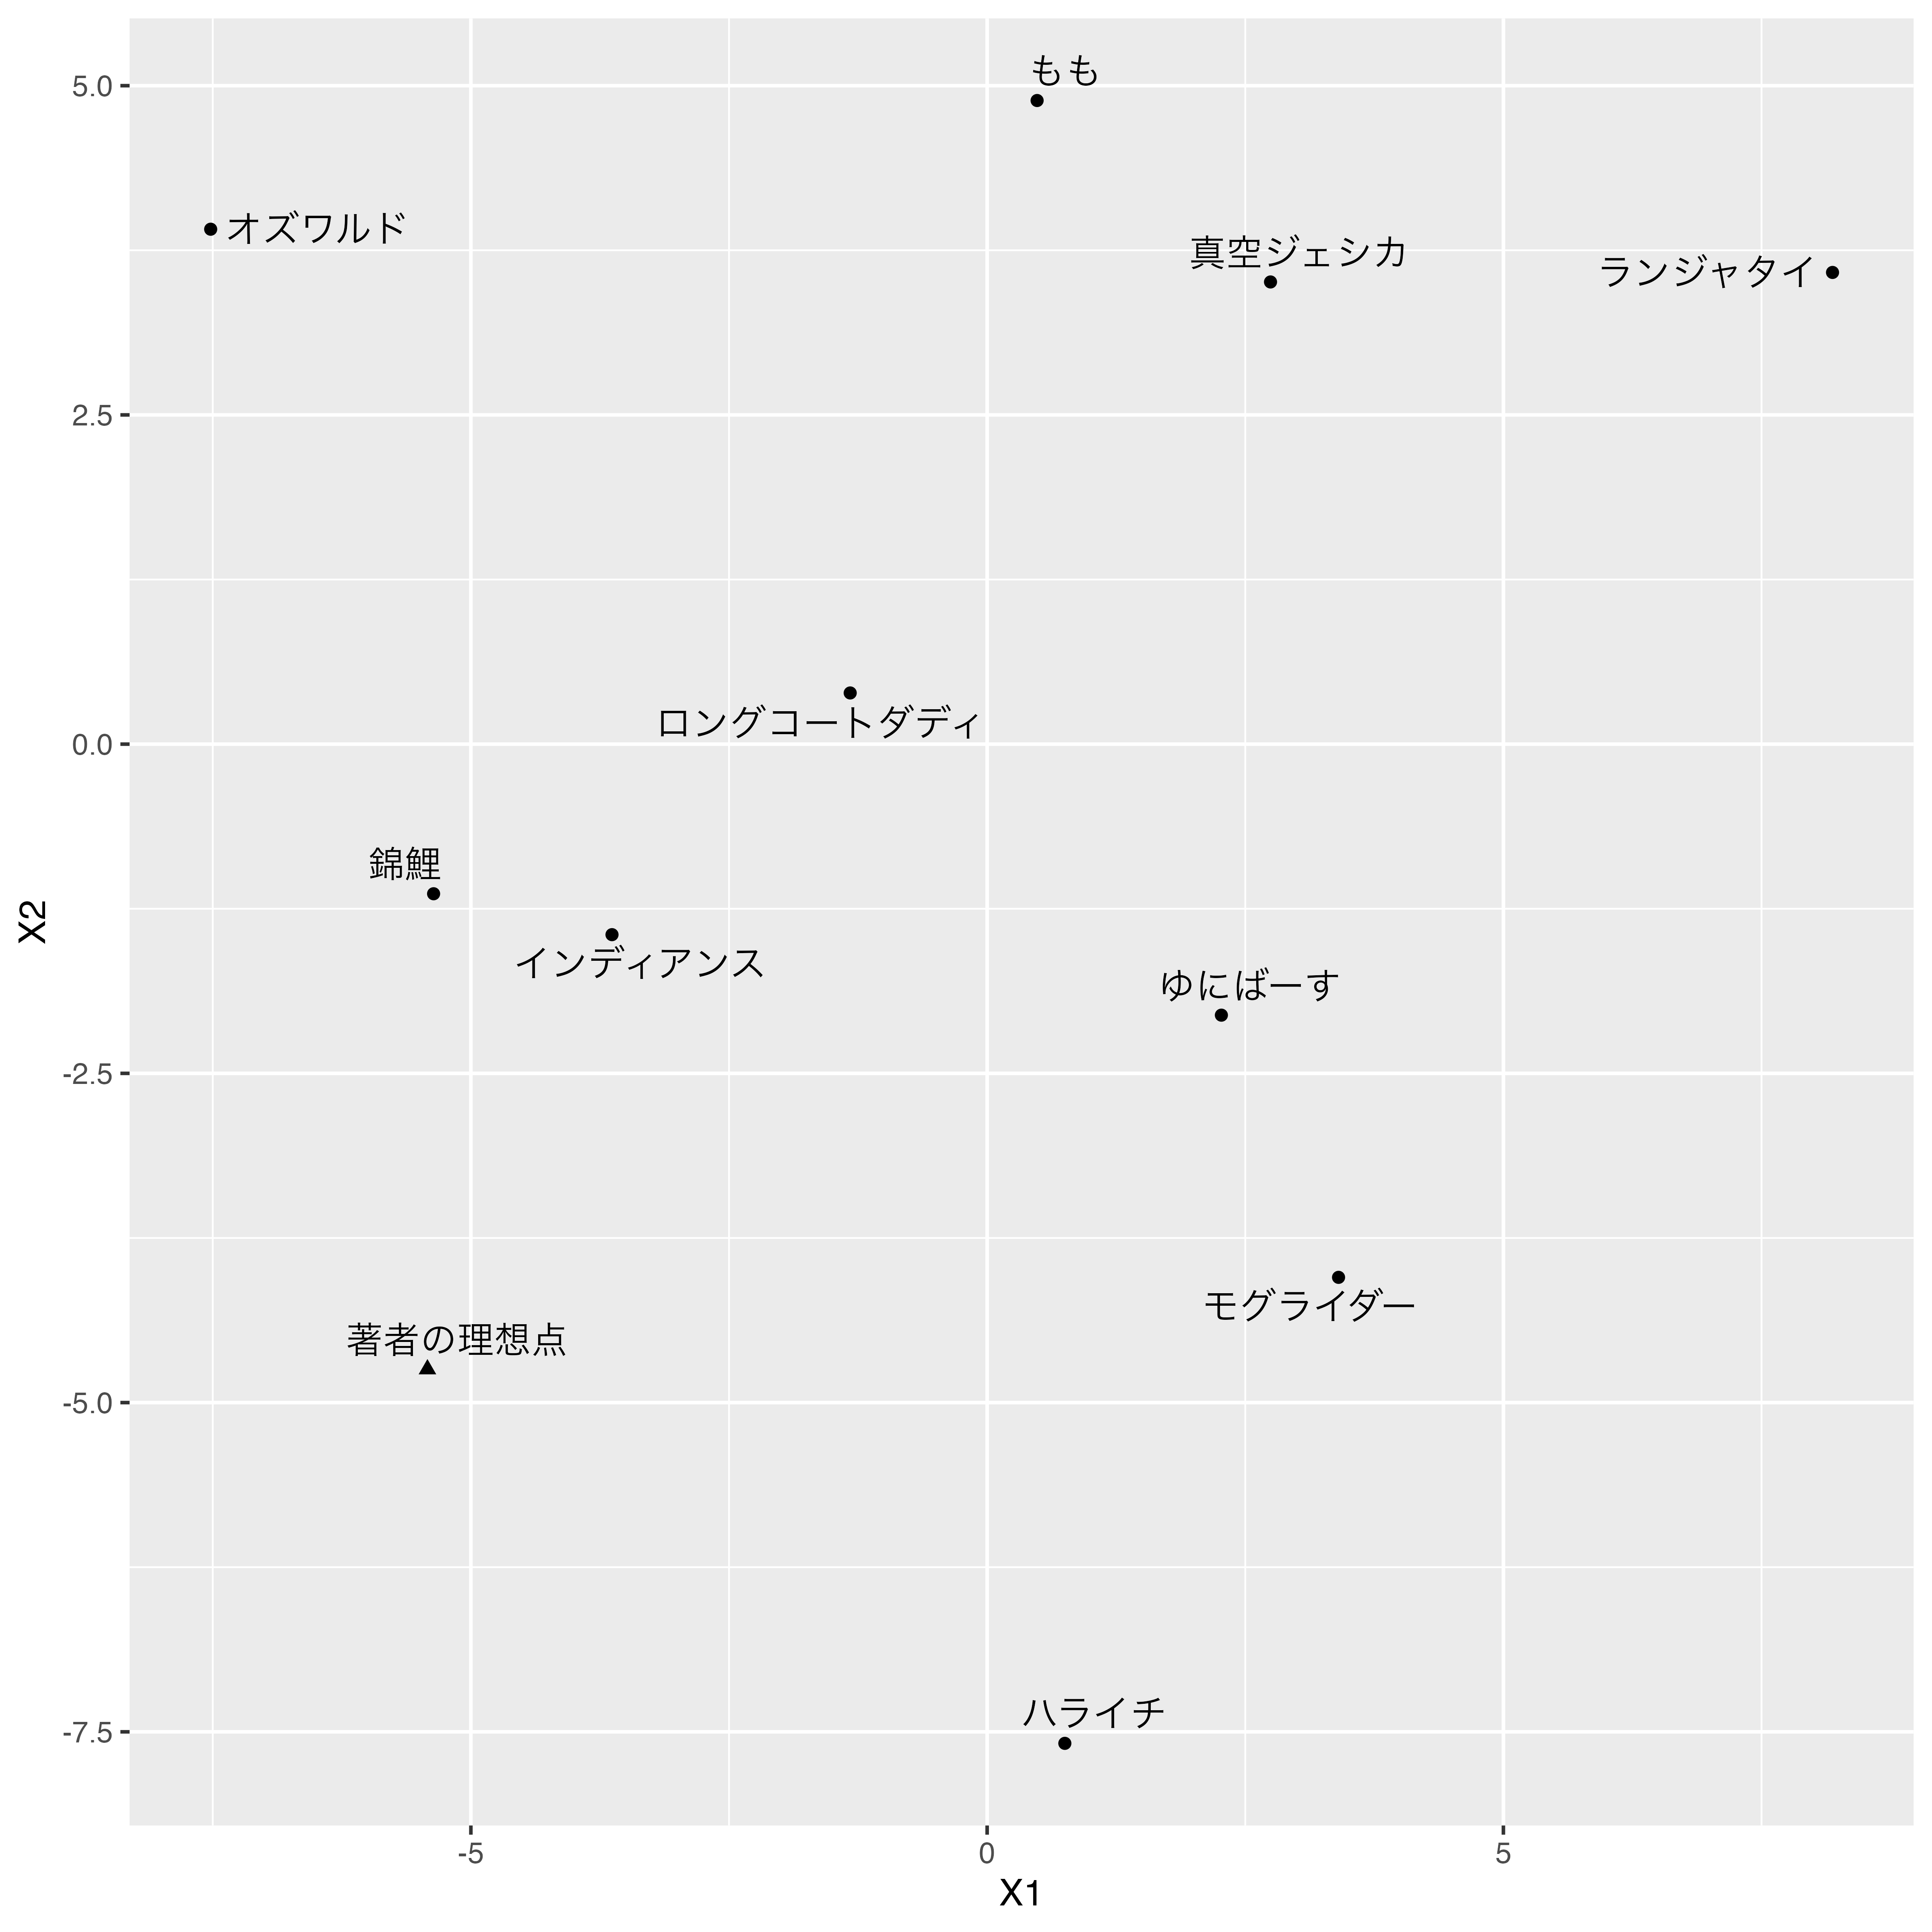
\includegraphics[width=0.8\linewidth,keepaspectratio]{../images/15_MDS/Rplot15_04.png}
		\caption{著者の理想点プロット}
		\label{fig:15_04}
	\end{center}
\end{figure}
\paragraph{Abelson Map}これは\textcite{abelson1954technique}の考えた手法で，これもprefmapと同じく布置される対象に別の力(選好度でもなんでもよい)があると考え，地図空間上に力の場をプロットして等高線を引くことで表現するモデルです。

この方法では，各点Pにかかる力$V(P)$を次のように定式化します。
\[ V(p) = \sum_{j=1}^M \frac{V(j)}{1+d_{pj}^2} \]
ここで$j$は各点，ここで言えば漫才師のことで，$V(j)$が漫才師$j$に与えられた評価点です。$d_{pj}^2$は任意の点$p$と対象$j$の距離ですから，任意の点$p$にかかる力は各漫才師が発する笑い力ですね。

この方法で，先ほどのM-1プロットに，著者の評価をAbelson Mapの方法で描き加えてみましょう。
\begin{figure}[ht]
	\begin{center}
		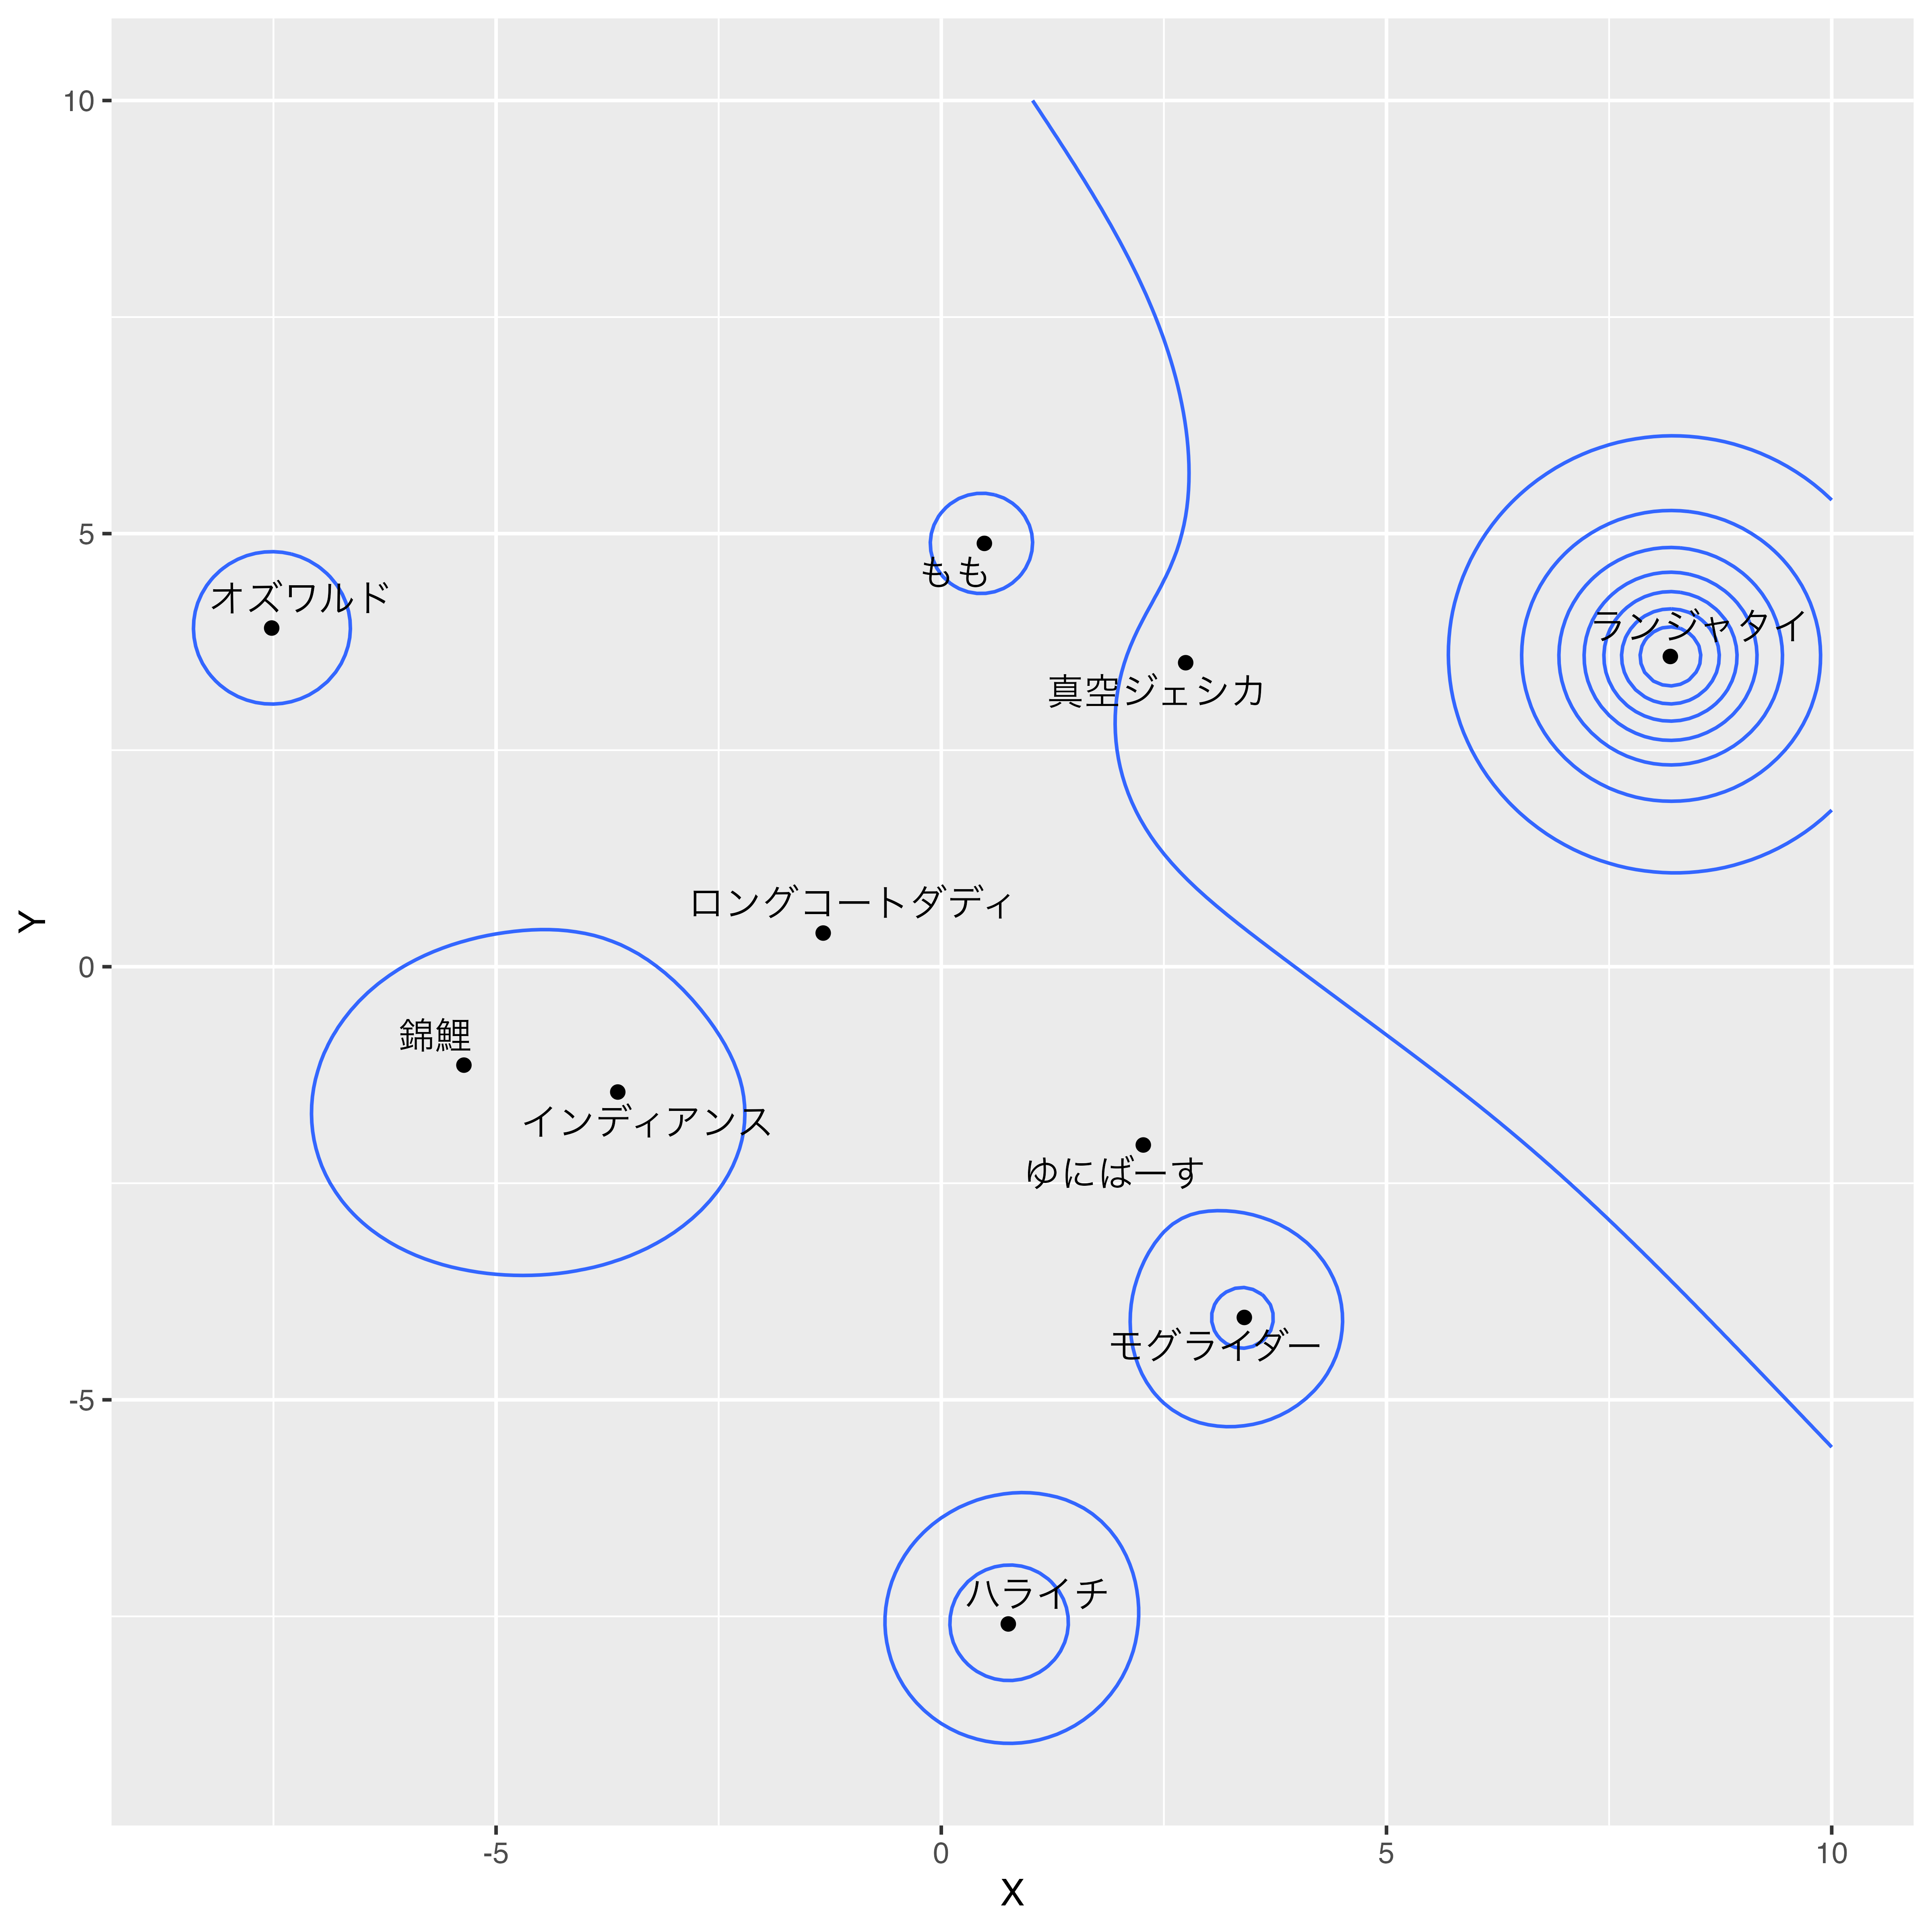
\includegraphics[width=0.8\linewidth,keepaspectratio]{../images/15_MDS/Rplot15_05.png}
		\caption{Abelson Mappingによるお笑い力の等高線図}
		\label{fig:15_05}
	\end{center}
\end{figure}
図\ref{fig:15_05}の右にある，ランジャタイの周りにたくさんの線が引かれていますが，いわばこれは低気圧のようにここのパワーが弱い(と著者は思っている)ところになります。実は，真空ジェシカの左側に通っているラインが平均点のラインですから，ここを境に著者は「面白い」と「面白くない」を区分しているとも言えます。ハライチやオズワルドの周りにある等高線は山の高さ，パワーの強さを表しているラインですね。

力のメタファーにすぎないと言われたらそうですが，このように色々なものを可視化できるのもMDSの面白いところです。

\paragraph{非対称多次元尺度構成法}距離データは対称でなければならない，というものの，たとえば好きな人に振り向いてもらえない＝片想いとか，都市間の人口の流入・流出，国際貿易の赤字・黒字などを考えると，対称間の関係が対称出ないことは少なくないわけです。そうした非対称な関係を，図に加えようと言うのが非対称MDSです。非対称情報を対象部分+歪対象部分に分割し，この対称でない要素を図の中に書き加えるモデルが一般的で，プロットする対象の周りに縁や楕円で表現するとか，矢印で表現するとか，vonMises分布と呼ばれる\keytermL{確率分布}{かくりつぶんぷ}で表現するとか，さきほどのAbelson Mapで高さとして表現するなどのモデルがあります。より数学的なモデルとして，プロットする空間を複素空間にするモデルもあります。詳しくは\textcite{Chino2012}を参考にしてください。

\paragraph{多次元展開法}リッカート法は心理尺度でもっともよく使われる方法で，「非常に当てはまる」から「まったく当てはまらない」までの段階的な反応を被験者に求める方法です。これは\keytermL{段階反応モデル}{だんかいはんのうもでる}で分析されることからも明らかなように，項目に対する反応段階が順番的に強くなっていくことを仮定しています。しかし，実際に被験者が丸をつけるときは，「自分の感覚にもっとも近いカテゴリーを選ぶ」ということをしているはずです。つまり，被験者と反応カテゴリーの距離が，尺度に反映されているはずなのです。この考え方から，尺度に対する反応を距離とし，項目とそれに回答した被験者の両方をプロットする地図を書く方法があります。Coombsが考えた\keyterm{多次元展開法}{たじげんてんかいほう}{Multi-dimensional unfolding method}と呼ばれる手法がそれで，この手法から態度測定の尺度化を考えることもできます。発想としては数量化理論に近く，また\textcite{shimizu2018}はこれを確率モデルに展開しています。

ここであげたいくつかの例にあるように，多次元尺度法もさまざまな角度から人の判断や反応から，\keyterm{尺度}{しゃくど}{scale}を作る方法です。多次元尺度構成法は因子分析モデルよりも制約や仮定が少なく，より直接的に心理的反応をモデル化しようとしています。

本講で学んだように，心理学ではさまざまな角度から「数値化するルール」を考えてきていますが，それぞれ仮定や目的，何を良い尺度と考えるかという観点がことなります。我々心理学者は，統計的なツールのユーザに過ぎません。データは分析できればそれでいい，分析は機械がやってくれるから深く考えなくていい，という割り切り方もあるかもしれませんが，「そもそも何をデータとするか」「どのように数値化するか」という点については，そのような態度は取れないはずです。なぜならそもそも「心はいかにして数値化できるか」ということが明らかでないならば，その後の分析はすべて嘘っぽい数字を使った統計ごっこに過ぎないからです。\textbf{心理学者であるために，われわれは何をどのように数値化しているかについて，しっかりと理解する必要があるのです。}

\section{課題}
計量MDS，非計量MDSをそれぞれ一例ずつ，実践してみてください。データはどのようなものでも構いません。提出ファイル形式はRスクリプトかRmdとします。なお提出されたコード単体でバグがなく動くことが確認できないものは，未提出扱いになります。コードの書き方などわからないところがあれば，曜日別TAか小杉までメールで連絡し，指導を受けてください。


\end{document}
